\documentclass[onlymath]{beamer}

%%%%%%%%%%%%%%%%%%%%%%%%%%%%%%%%%%%%%%%%%%%%%%%%%%%%%%%%%%%%%%%%%%%%%
% COLORES
%%%%%%%%%%%%%%%%%%%%%%%%%%%%%%%%%%%%%%%%%%%%%%%%%%%%%%%%%%%%%%%%%%%%%
\usepackage{color}

\definecolor{titulo}{HTML}{750202}

\definecolor{seccion}{HTML}{360101}
\definecolor{sombra_seccion}{HTML}{750202}

\definecolor{subseccion}{HTML}{750202}
\definecolor{sombra_subseccion}{HTML}{A75E5E}

\definecolor{listas}{HTML}{750202}

\definecolor{tb-std}{HTML}{360101}
\definecolor{tb-ale}{HTML}{02020A}
\definecolor{tb-exa}{HTML}{02020A}
\definecolor{fb-std}{HTML}{A75E5E}
\definecolor{fb-ale}{HTML}{d01800}
\definecolor{fb-exa}{HTML}{fee8ef}
\definecolor{cb-std}{HTML}{fee8ef}
\definecolor{cb-ale}{HTML}{fee8ef}
\definecolor{cb-exa}{HTML}{fff2f2}

\definecolor{primero}{HTML}{fee8ef}
\definecolor{segundo}{HTML}{ffe8ef}
\definecolor{tercero}{HTML}{ffe8ee}
\definecolor{cuarto}{HTML}{ffecf1}
\definecolor{quinto}{HTML}{fff0f4}

%%%%%%%%%%%%%%%%%%%%%%%%%%%%%%%%%%%%%%%%%%%%%%%%%%%%%%%%%%%%%%%%%%%%%
% TEMA
%%%%%%%%%%%%%%%%%%%%%%%%%%%%%%%%%%%%%%%%%%%%%%%%%%%%%%%%%%%%%%%%%%%%%
\useinnertheme{circles} % Tipo de tema para el índice
\setbeamertemplate{itemize items}[triangle]
\setbeamertemplate{enumerate items}[default]
\setbeamerfont{title}{size = \huge}
\setbeamerfont{frametitle}{size = \Large}
\setbeamercolor{normal text}{fg = black} % Color del texto
\setbeamercolor{frametitle}{fg = titulo} % Color del título de las diapositivas
\setbeamercolor{title}{fg = titulo} % Color del título de la presentación
\setbeamercolor{section in toc}{fg = seccion} % Color de la sección actual
\setbeamercolor{section in toc shaded}{fg = sombra_seccion} % Color de la sección sombreada
\setbeamercolor{subsection in toc}{fg = subseccion} % Color de la subsección actual
\setbeamercolor{subsection in toc shaded}{fg = sombra_subseccion} % Color de la subsección sombreada
\setbeamercolor{item}{fg = listas} % Color de los ítems
\setbeamercolor{subitem}{fg = listas} % Color de los subítems
\setbeamercolor{subsubitem}{fg = listas} % Color de los subsubítems
\setbeamercolor{description item}{fg = listas} % Color del título de los ítems en las descripciones
\setbeamercolor{caption}{fg = black} % Color de las etiquetas
\setbeamercolor{caption name}{fg = black} % Color de las etiquetas
% Bloque estándar
\setbeamercolor{block title}{fg = tb-std, bg = fb-std} % Título del bloque
\setbeamercolor{block body}{bg = cb-std} % Cuerpo del bloque
% Bloque Alert
\setbeamercolor{block title alerted}{fg = tb-ale, bg = fb-ale} % Título del bloque
\setbeamercolor{block body alerted}{bg = cb-ale} % Cuerpo del bloque
% Bloque Example
\setbeamercolor{block title example}{fg = tb-exa, bg = fb-exa} % Título del bloque
\setbeamercolor{block body example}{bg = cb-exa} % Cuerpo del bloque

%%%%%%%%%%%%%%%%%%%%%%%%%%%%%%%%%%%%%%%%%%%%%%%%%%%%%%%%%%%%%%%%%%%%%
% PREÁMBULOS
%%%%%%%%%%%%%%%%%%%%%%%%%%%%%%%%%%%%%%%%%%%%%%%%%%%%%%%%%%%%%%%%%%%%%
\AtBeginSubsection[] % Índice al principio de cada subsección
{
  \begin{frame}
    \frametitle{Índice de contenidos}
    \tableofcontents[currentsection,currentsubsection]
  \end{frame}
}

%%%%%%%%%%%%%%%%%%%%%%%%%%%%%%%%%%%%%%%%%%%%%%%%%%%%%%%%%%%%%%%%%%%%%
% MISCELÁNEO
%%%%%%%%%%%%%%%%%%%%%%%%%%%%%%%%%%%%%%%%%%%%%%%%%%%%%%%%%%%%%%%%%%%%%
\beamertemplatenavigationsymbolsempty % Elimina la barra de navegación
\usepackage[T1]{fontenc}
\usepackage{antpolt}
\usepackage[spanish]{babel}
\usepackage{graphicx} % Insertar imágenes
\renewcommand{\figurename}{Figura} % Cambiar el título de las etiquetas de las figuras


%%%%%%%%%%%%%%%%%%%%%%%%%%%%%%%%%%%%%%%%%%%%%%%%%%%%%%%%%%%%%%%%%%%%%
% PORTADA
%%%%%%%%%%%%%%%%%%%%%%%%%%%%%%%%%%%%%%%%%%%%%%%%%%%%%%%%%%%%%%%%%%%%%
\title{\textbf{COLONOS DE CATAN}}
\subtitle{Guía estratégica}
\author{\textit{Manuel Gachs Ballegeer}}
\date{2020 d.C.}

%%%%%%%%%%%%%%%%%%%%%%%%%%%%%%%%%%%%%%%%%%%%%%%%%%%%%%%%%%%%%%%%%%%%%
% DOCUMENTO
%%%%%%%%%%%%%%%%%%%%%%%%%%%%%%%%%%%%%%%%%%%%%%%%%%%%%%%%%%%%%%%%%%%%%

\usepackage{graphicx}
\begin{document}
\frame{
	\maketitle
}
\section{Conceptos básicos}
\subsection{Clasificación de los recursos}
\frame{
	\frametitle{El espacio vectorial $P_R$}
		En Catan existen cinco recursos distintos, que denominaremos de la
		siguiente manera:
		\begin{block}{}
		\centering
		madera := $m$, arcilla := $a$, trigo := $t$, ovejas := $g$, 
		piedra := $p$
		\end{block}
		\begin{figure}[htp]
\centering
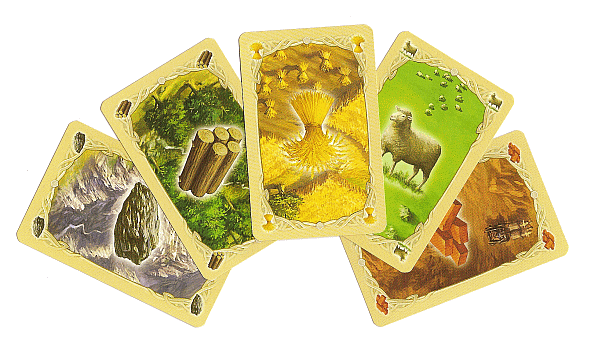
\includegraphics[scale=0.35]{recursos_catan.png}
\end{figure}
}
\frame{
	Podemos definir los siguientes conjuntos:
	$$R := \{m,a,t,g,p\}$$
	$$P_R := \Bigg\{\sum_{\substack{i=1\\r\in R}}^5k_ir,\;k_i\in\mathbb{N}
	\Bigg\}$$
	donde el conjunto $P_R$ representa las posibles manos que puede tener 
	un jugador.
	\begin{block}{}
		El conjunto $P_R$ tiene estructura de espacio vectorial, y 
		$P_R=\mathcal{L}(R)$
	\end{block}
}
\frame{
	\frametitle{Construcciones}
	\begin{columns}
		\begin{column}{.5\textwidth}
			Las distintas construcciones de Catan pueden verse como elementos 
			de $P_R$, y son las siguientes:
			\begin{itemize}
				\item \emph{Carretera}: $v = (1,1,0,0,0)$
				\item \emph{Poblado}: $p=(1,1,1,1,0)$
				\item \emph{Ciudad}: $c=(0,0,2,0,3)$
				\item \emph{Desarrollo}: $d=(0,0,1,1,1)$
			\end{itemize}
		\end{column}
		\begin{column}{.5\textwidth}
			\begin{figure}[htp]
			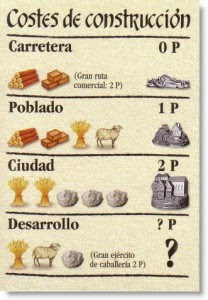
\includegraphics[scale=0.50]{costes_catan.jpg}
			\end{figure}
		\end{column}
	\end{columns}
}
\frame{
	\frametitle{Puntuación de las construcciones}
	Cada construcción nos otorga una cantidad de puntos.
	\begin{exampleblock}{\textbf{Carretera}}
	La carretera en si misma no nos otorga puntos, pero como son necesarias
	al menos dos para construir un poblado, entonces diremos que dan $^1/_3$ 
	de un punto.
	\end{exampleblock}
	\begin{exampleblock}{\textbf{Poblado}}
	El poblado otorga un (1) punto.
	\end{exampleblock}
	\begin{exampleblock}{\textbf{Ciudad}}
	La ciudad otorga dos puntos, pero al tener que construirla sobre un 
	poblado, realmente otorga un (1) punto.
	\end{exampleblock}
}
\frame{
	\begin{exampleblock}{\textbf{Desarrollo}}
	Entre las cartas de desarrollo (25) existen cinco cartas de puntos. 
	Además, con tres caballeros (14 en total) obtienes dos puntos. Por tanto,
	una carta de desarrollo otorga $\frac{5}{25}+\frac{14\cdot 13\cdot 12}
	{25\cdot 24\cdot 23}=\frac{297}{575}$ de un punto.
	\end{exampleblock}
	\begin{figure}[htp]
	\centering
	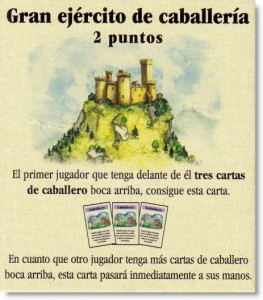
\includegraphics[scale=0.40]{gran_ejercito_caballeria.jpg}
	\end{figure}
}
\frame{
	\frametitle{Clasificación de los recursos por puntuación esperada}
	Definamos una aplicación $\varphi:R\to\mathbb{R}$. Esta apliación la 
	usaremos para dar un valor numérico a cada recurso, con lo que podremos
	clasificarlos en un orden de importancia. Definimos también el conjunto
	de construcciones $C=\{c_1=v,c_2=p,c_3=c,c_4=d\}$.
	$$\varphi(r) = \frac{\sum_{i=1}^4[(\text{puntos de }c_i)\cdot
	(\text{valor de la componente }r\text{ en }c_i)]}
	{\text{hexágonos con el recurso }r}$$
	Obtenemos por tanto los siguientes valores:
	\begin{itemize}
		\item \emph{Madera}: $\varphi(m)\approx 0,333$
		\item \emph{Arcilla}: $\varphi(m)\approx 0,444$
		\item \emph{Trigo}: $\varphi(m)\approx 0,629$
		\item \emph{Ovejas}: $\varphi(m)\approx 0,379$
		\item \emph{Piedra}: $\varphi(m)\approx 1,172$
	\end{itemize}
}
\frame{
	En conclusión, obtenemos la siguiente clasificación por puntuación 
	esperada:
	\\
	\centering
	\begin{tabular}{c}
	{\color{titulo}{1.}} Piedra \\
	{\color{titulo}{2.}} Trigo \\
	{\color{titulo}{3.}} Arcilla \\
	{\color{titulo}{4.}} Ovejas \\
	{\color{titulo}{5.}} Madera \\
	\end{tabular}
	\bigskip
	\begin{alertblock}{Nota importante}
	Aunque la puntuación esperada de las ovejas es mayor que la de la madera,
	sin madera es imposible desarrollar la economía al principio de la 
	partida.
	\end{alertblock}
}
\subsection{Reglas de los números}
\frame{
	\frametitle{Reglas de los números}
	\begin{figure}[htp]
	\centering
	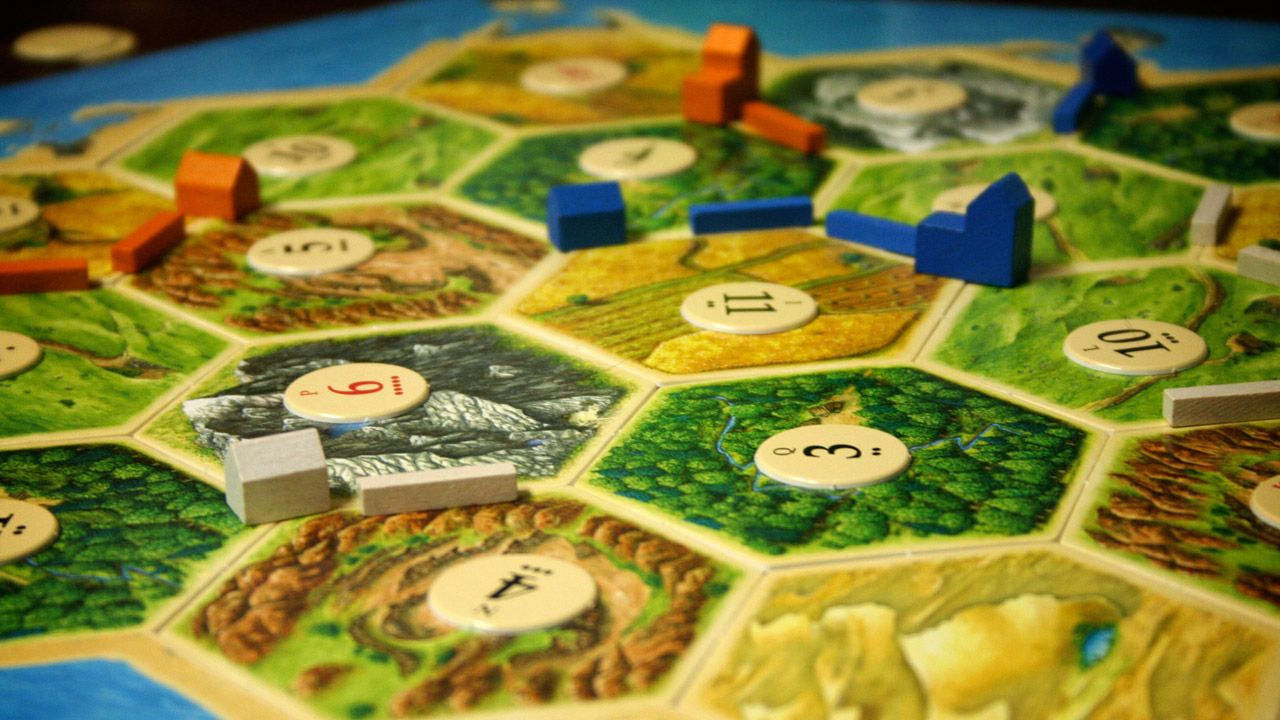
\includegraphics[scale=0.20]{mapa_catan.jpg}
	\end{figure}
	Los números sobre cada hexágono son muy importantes, puesto que no todos
	tienen la misma probabilidad de salir. Existen dos reglas generales
	sobre los números a la hora de posicionarse:
}
\frame{
	\begin{block}{Regla del más probable}
		Una posición es mejor que otra si cada uno de los números de los 
		hexágonos que comparten ese vértice se acercan más al número 7.
	\end{block}
	\begin{block}{Regla de la diversidad numérica}
		Una posición es mejor que otra si comparte menos números con el resto
		de posiciones del jugador.
	\end{block}
	El sentido de la diversidad numérica es muy simple. Cuantos más números
	distintos tengamos, mayores las posibilidades de obtener recursos.
}
\subsection{Los puertos}
\frame{
	\frametitle{La importancia de los puertos}
	Los puertos son \textbf{extremadamente importantes} para la economía de
	la partida:
	\begin{itemize}
		\item Mejoran los intercambios con el banco.
		\item Permiten un cierto grado de ``autarquía''.
		\item Presionan comercialmente al resto de jugadores.
		\item Pueden ser la pieza central de una estrategia.
	\end{itemize}
	Es recomendable que al menos una de las dos posiciones iniciales estén a
	rango de un puerto, y a ser posible uno de 3:1.
}
\subsection{Los jugadores y el posicionamiento}
\frame{
	\frametitle{Diferencias entre partidas de 3 y 4 jugadores}
	Existen diferencias sustanciales entre las partidas de tres jugadores y
	las de cuatro. Esas diferencias provocan que algunas estrategias sean más
	o menos viables dependiendo de los jugadores. Algunas de las diferencias
	son las siguientes (algunas son consecuencias de otras):
	\begin{itemize}
		\item En partidas de cuatro jugadores, un jugador suele quedarse
		rezagado en cuanto a puntos con los demás jugadores.
		\item Las partidas de cuatro jugadores apenas permiten el 
		expansionismo.
		\item La importancia del orden de posicionamiento es menor en partidas
		de tres jugadores.
	\end{itemize}
}
\frame{
	\frametitle{El posicionamiento inicial}
	En cuanto al orden, es mejor ser o el \textbf{primero} o el 
	\textbf{último}.
	\begin{columns}
		\begin{column}{.5\textwidth}
			\begin{exampleblock}{Ventaja del primero}
				Tienes la mejor posición inicial.
			\end{exampleblock}
			\begin{exampleblock}{Ventaja del último}
				Pones los dos poblados a la vez.
			\end{exampleblock}
		\end{column}
		\begin{column}{.5\textwidth}
			\begin{figure}[htp]
			\centering
			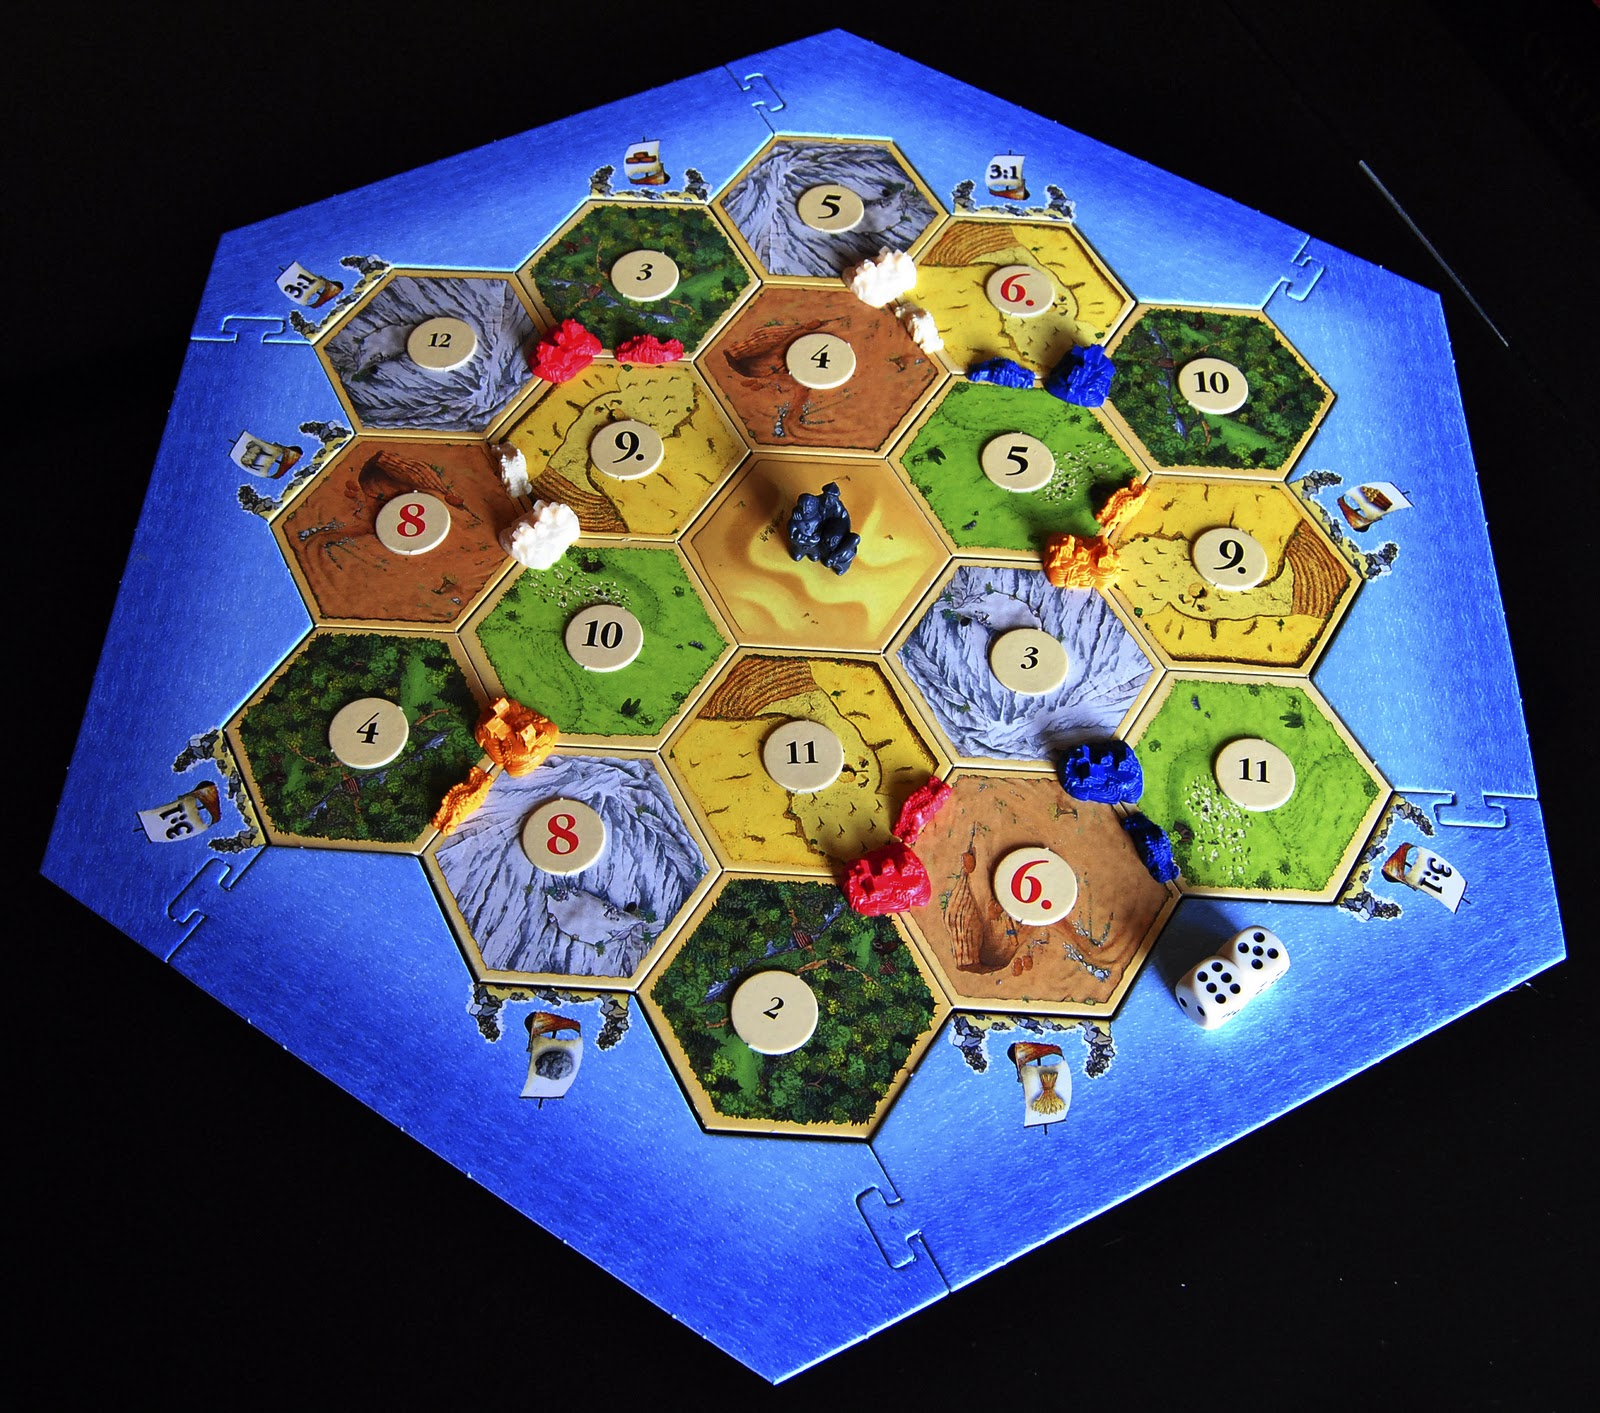
\includegraphics[scale=0.09]{inicio_4p.jpg}
			\end{figure}
		\end{column}
	\end{columns}
}
\frame{
	\frametitle{Ejemplo 1}
}
\frame[plain]{
}
\frame{
	\frametitle{Ejemplo 2}
}
\frame[plain]{
}
\section{Conceptos avanzados}
\subsection{Sacrificar recursos}
\frame{
	\frametitle{Sacrificar recursos}
	En ocasiones, es imposible (o no nos interesa) tener acceso a todos los
	recursos desde el inicio de la partida. A la hora de sacrificar uno de 
	los recursos, debemos responder a las siguientes preguntas:
	\begin{itemize}
		\item \textquestiondown Lo necesito para poder hacer algo el primer
		turno?
		\item \textquestiondown Puedo obtenerlo de alguna otra manera?
		\item \textquestiondown Tengo a rango alguna fuente de ese recurso?
	\end{itemize}
	Dependiendo de la situación la respuesta puede cambiar; pero, en general,
	la respuesta suele ser las \textbf{ovejas}.
}
\subsection{El comercio}
\section{Estrategias}
\subsection{La estrategia de las cuatro ciudades}
\subsection{La estrategia del colono}
\subsection{La estrategia del monopolio}
\subsection{La estrategia de los 3 puntos}
\subsection{Ejemplos prácticos}
\end{document}